
\begin{table}
    \centering
        \begin{tabular}{l l l l l}
        \toprule
        Setting & PIQA & ARC (Easy) & ARC (Challenge) & OpenBookQA \\ 
        \midrule
        Fine-tuned SOTA & 79.4 & \textbf{92.0}\cite{khashabi2020unifiedqa} & \textbf{78.5}\cite{khashabi2020unifiedqa}  & \textbf{87.2}\cite{khashabi2020unifiedqa}  \\ 
        GPT-3 Zero-Shot  & \textbf{80.5}* & 68.8 & 51.4 & 57.6 \\
        GPT-3 One-Shot & \textbf{80.5}* & 71.2 & 53.2 & 58.8 \\
        GPT-3 Few-Shot & \textbf{82.8}* & 70.1 & 51.5 &  65.4 \\
        \bottomrule
        \end{tabular}
    \caption{GPT-3 results on three commonsense reasoning tasks, PIQA, ARC, and OpenBookQA. GPT-3 Few-Shot PIQA result is evaluated on the test server.  See Section \ref{section:measuring_and_preventing_memorization_of_benchmarks} for details on potential contamination issues on the PIQA test set.}
    \label{table:reasoning}
\end{table}
\begin{figure}
\centering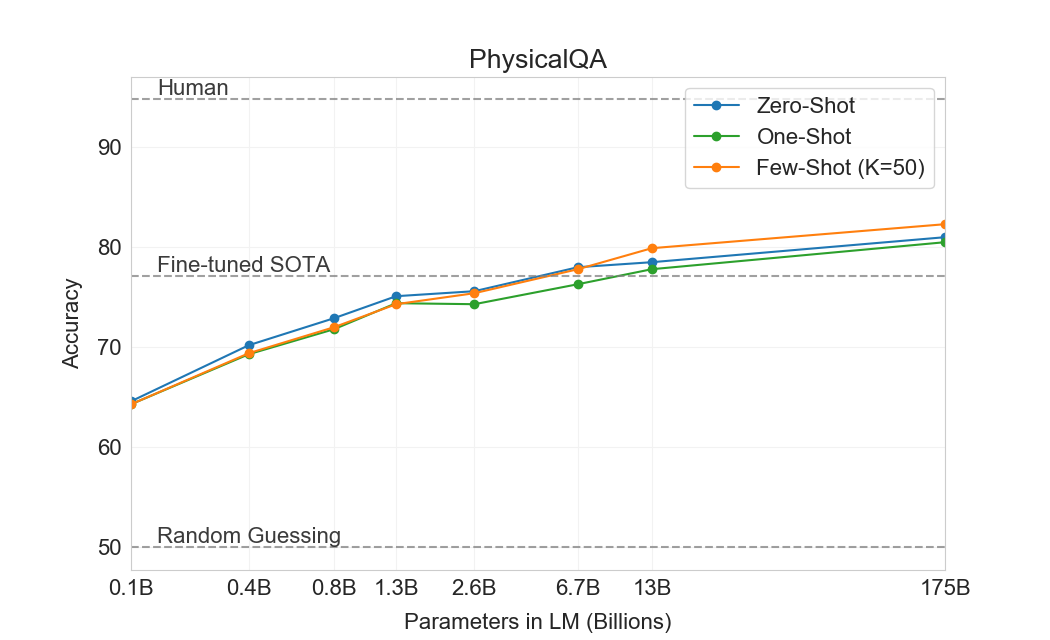
\includegraphics[width=0.8\linewidth]{graphs/scale_plots/piqa.png}
\caption{GPT-3 results on PIQA in the zero-shot, one-shot, and few-shot settings. The largest model achieves a score on the development set in all three conditions that exceeds the best recorded score on the task.}
\label{graph:physicalqa}
\end{figure}
Next we consider three datasets which attempt to capture physical or scientific reasoning, as distinct from sentence completion, reading comprehension, or broad knowledge question answering. The first, PhysicalQA (PIQA) \cite{bisk2019piqa}, asks common sense questions about how the physical world works and is intended as a probe of grounded understanding of the world. GPT-3 achieves 81.0\% accuracy zero-shot, 80.5\% accuracy one-shot, and 82.8\% accuracy few-shot (the last measured on PIQA's test server).  This compares favorably to the 79.4\% accuracy prior state-of-the-art of a fine-tuned RoBERTa. PIQA shows relatively shallow scaling with model size and is still over 10\% worse than human performance, but GPT-3's few-shot and even zero-shot result outperform the current state-of-the-art.  Our analysis flagged PIQA for a potential data contamination issue (despite hidden test labels), and we therefore conservatively mark the result with an asterisk. See Section \ref{section:measuring_and_preventing_memorization_of_benchmarks} for details.

ARC \cite{Clark2018ThinkYH} is a dataset of multiple-choice questions collected from 3rd to 9th grade science exams. On the ``Challenge'' version of the dataset which has been filtered to questions which simple statistical or information retrieval methods are unable to  correctly answer, GPT-3 achieves 51.4\% accuracy in the zero-shot setting, 53.2\% in the one-shot setting, and 51.5\% in the few-shot setting. This is approaching the performance of a fine-tuned RoBERTa baseline (55.9\%) from UnifiedQA \cite{khashabi2020unifiedqa}. On the ``Easy'' version of the dataset (questions which either of the mentioned baseline approaches answered correctly), GPT-3 achieves 68.8\%, 71.2\%, and 70.1\% which slightly exceeds a fine-tuned RoBERTa baseline from \cite{khashabi2020unifiedqa}. However, both of these results are still much worse than the overall SOTAs achieved by the UnifiedQA which exceeds GPT-3’s few-shot results by 27\% on the challenge set and 22\% on the easy set.

On OpenBookQA \cite{Mihaylov2018CanAS}, GPT-3 improves significantly from zero to few shot settings but is still over 20 points short of the overall SOTA. GPT-3's few-shot performance is similar to a fine-tuned BERT Large baseline on the leaderboard.

Overall, in-context learning with GPT-3 shows mixed results on commonsense reasoning tasks, with only small and inconsistent gains observed in the one and few-shot learning settings for both PIQA and ARC, but a significant improvement is observed on OpenBookQA. GPT-3 sets SOTA on the new PIQA dataset in all evaluation settings.

